%%%%%%%%%%%%%%%%%%%%%%%%%%%%%%%%%%%%%%%%%%%%%%%%%%%%%%%%%%%
%
%        
%
%\documentclass[letterpaper, 10 pt, conference]{ieeeconf}  % Comment this line out if you need a4paper
%
\documentclass[a4paper, 10pt, conference]{ieeeconf}      % Use this line for a4 paper
%
%\IEEEoverridecommandlockouts                              % This command is only needed if 
                                                          % you want to use the \thanks command
%
\overrideIEEEmargins                                      % Needed to meet printer requirements.
%
% See the \addtolength command later in the file to balance the column lengths
% on the last page of the document
%
\usepackage{graphicx} % for pdf, bitmapped graphics files
%\usepackage{hyperref}
%\hypersetup{colorlinks,urlcolor=blue,linkcolor=blue}
%
\usepackage{epstopdf}
%\usepackage{mathptmx} % assumes new font selection scheme installed
%\usepackage{times} % assumes new font selection scheme installed
\usepackage{amsmath} % assumes amsmath package installed
\usepackage{amssymb}  % assumes amsmath package installed
\usepackage{graphicx}
%\usepackage{subfig}
\usepackage{caption}
\usepackage{subcaption}
\usepackage{array}
\usepackage[space]{cite}
%\usepackage[hidelinks]{hyperref}
\usepackage[colorlinks, linkcolor = black, citecolor = black, filecolor = black, urlcolor = blue]{hyperref}
\usepackage{lscape} %% landscape
\usepackage{longtable} %% big table
\usepackage{tikz}

\newcommand\encircle[1]{%
	\tikz[baseline=(X.base)] 
	\node (X) [draw, shape=circle, inner sep=0.5pt] {#1};}





%\DeclarePairedDelimiter\abs{\lvert}{\rvert}%
%\DeclarePairedDelimiter\norm{\lVert}{\rVert}%
\DeclareMathOperator*{\argmin}{argmin}
\DeclareMathOperator*{\argmax}{argmax}
\DeclareMathOperator*{\sgn}{sgn}
\newcommand{\specialcell}[2][c]{%
	\begin{tabular}[#1]{@{}c@{}}#2\end{tabular}}

\renewcommand{\citedash}{--}


\newcommand{\etal}{~\textit{et al.}}
%
\title{\bf {\LARGE Mechanisms and Sensors for Robotic Fingers} \\
{\normalsize H$^2$T-Seminar: Humanoid Robotics, WS 18/19}}
\author{Shant Gananian, Pascal Weiner and Tamim Asfour \\ High Performance Humanoid Technologies \\ Institute for Anthropomatics and Robotics \\ Karlsruhe Institute of Technology \\
\url{http://www.humanoids.kit.edu}}


%
%
\begin{document}
\maketitle
\thispagestyle{plain}
\pagestyle{plain}
%
%%%%%%%%%%%%%%%%%%%%%%%%%%%%%%%%%%%%%%%%%%%%%%%%%%%%%%%%%%%%%%%%%%%%%%%%%%%%%%%%
\begin{abstract}
: In the past years robotics has matured from being mostly used in the industry and made a break into our daily lives. Similarly, the research focus for grasping and manipulation has evolved from manipulators and grippers to dexterous anthropomorphic hands, capable of performing different tasks in unstructured environment.
The fingers of these hands play a crucial role in their success and performance. Designing these fingers opens researchers to many considerations to choose the best suitable specifications for the fingers, some of which will be discussed in this paper.
\end{abstract}

%%%%%%%%%%%%%%%%%%%%%%%%%%%%%%%%%%%%%%%%%%%%%%%%%%%%%%%%%%%%%%%%%%%%%%%%%%%%%%%%
\section{\textbf{Introduction}}
The idea of copying the human hand is so old and may be contemporary of the first automata in the 18th century, e.g., La Musicienne of the inventor Jacquet-Droz \cite{birglen2007underactuated}. This automate was able to play a wide variety of organ partitions with two five-finger hands actuated with steel cables connected to a programming cam shaft.\\
The human hand has been an inspiration for robotic hand designers for decades. The first robotic hand, as it is commonly referred to, was perhaps the end-effector of the Handyman, a robot developed by Ralph Mosher for General Electric in 1960. Around 1969, the first research projects on robotic hands with three fingers including a “thumb” in opposition —hence an anthropomorphic design— began in the United States and in Japan.\\
For a prosthetic hand the focus is much more on aesthetics, weight and broad range of functionality, while the supply of power is limited, so self-locking mechanisms are preferred. Today's prosthetic hands have integrated drive technologies and weigh less than 500 g; The average human hand is around 0.58\% of the total body weight (approximately 400g).\\
Because of the dexterity of the human hand, many recent humanoid robots research projects addressed in their designs the anthropomorphism of the robotic hand. Many research laboratories around the world have developed prototypes of such hands as early as in the mid 1980’s when the foundations of these studies were laid (Mason and Salisbury 1985), by taking the human hand as a model for the robotic manipulation, in terms of performance and versatility.\\
The dexterity of robots has always been clearly more limited than that of a well-trained human being.\\
In fact we can find anthropomorphic end-effectors with very poor dexterity level, even if they are called hands, they perform very rough grasping procedures. Similarly, we can find smart end-effectors, capable of sophisticated manipulation procedures, but without any level of anthropomorphism.\\
Anthropomorphism is not necessary for achieving dexterity, and nor sufficient. But still it is desirable goal in the design of robotic end-effectors in operating in an environment where tasks may be executed by a robot or by a man, or in tele-operation of the end-effector by a man, or when it is required that the robot has human-like aspects and behavior. Considering that the human hand is capable of prehension (grasping objects of different size and shape) and apprehension (understanding through active touch), then it is both an output and input device. It can apply forces and provide information about the state of the interaction with the object. These characteristics are desirable in advanced robot hands.\\
%%%%%%%%%%%%%%%%%%%%%%%%%%%%%%%%%%%%%%%%%%%%%%%%%%%%%%%%%%%%%%%%%%%%%%%%%%%%%%%%
\section{\textbf{Robotic Fingers}}
Fingers of the hand are organs of manipulation and sensation. They move in the following ways: flexion, extension, abduction and adduction.\\
The anatomy of fingers in nature shows us the following design characteristics:\\
\begin{itemize}
	\item A serial bone-link structure mainly for rigidity and load capability.
	\item An actuation muscle system aiming to rotate each bone-link independently but with coordinate movements with other finger links.\\
\end{itemize}
Human hands have a highly articulated thumb. Amputation of the thumb is cited to cause 40\% loss of hand function and around 20\% disability of the whole person. The main motions of the thumb are flexion, extension, abduction/adduction and opposition. The thumb facilitates the grasping tasks by means of these motions.\\
Designing fingers to accomplish assigned tasks is a complex procedure.\\
In general common requirements can be identified mainly in the aspects for:\\
\begin{enumerate}
  \item Motion properties in:
  	\begin{itemize}
  		\item Grasping configurations
  		\item Smooth approaching motion
		\item Adaptable motion configuration to object shapes
		\item Reconfigurable grasping configurations
		\item Workspace ranges
		\item Limited motion impacts again objects to be grasped
	\end{itemize}
  \item Force capability in:
  	\begin{itemize}
  		\item Stable grasping configurations
		\item Efficient transmission of input power to grasping forces
		\item Distribution of grasping forces among several contacts with grasped object
		\item Positions of application points of the grasping forces
		\item Adjustable grasping forces
  	\end{itemize}
  \item Mechanical design in:
  	\begin{itemize}
  		\item Stiff or compliant structure at grasp
		\item Phalanx shape for adaptability to object shape
		\item Room for sensors
		\item Compact design versus human-like solutions
		\item Lightweight solution with smart or traditional materials
		\item Low-friction joints
		\item Location of power source\\
  	\end{itemize}
\end{enumerate}
Some of the key issues considered by developers or researchers when choosing the fingers specifications are:\\
	\begin{itemize}
		\item Number of Fingers
		\item Shape of the fingertips
		\item Compliant joints
		\item Built-in or remote actuation
		\item Transmission systems
		\item Sensors
		\item Materials and manufacturing\\
	\end{itemize}
%%%%%%%%%%%%%%%%%%%%%%%%%%%%%%%%%%%%%%%%%%%%%%%%%%%%%%%%%%%%%%%%%%%%%%%%%%%%%%%%
\section{\textbf{Number of Fingers}}
Number of fingers in anthropomorphic robotic hands can differ, but increased number of fingers provide a larger grasping surface and increases conformity to shapes.\\
A comparison chart for robotic hands researched and developed between the years of 1979 to 2016 is presented in the Table \ref{hand-comparison}\\
By reviewing dexterous robotic hands developed between 1983 to 2016 \cite{ramirez20173} it was visible that the five finger configuration is superior over the three or four finger setups (Fig.\ref{fig:DistributionOfFingerConfigurations}).\\
It was assumed that this trend is due to the fact that the robots are moving to more dynamic and human populated scenarios, where unlike the industrial grippers the new applications don't measure the effectiveness only in terms of repetition and high precision. Many studies used hands with different finger configurations for different applications with positive results. One does not overcome the other, though their purposes and applications might be different.\\
Due to their more available postures, the five finger hands can provide more flexibility and grasping postures compared to the traditional grippers, but it is also more complex.\\
The correct hand is dependent upon the tasks to be done and the environment in which such activities take place.\\
\begin{figure}[h!]
\centering  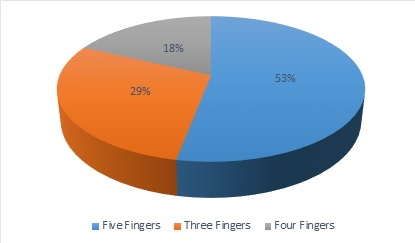
\includegraphics[width=1.0\linewidth]{./images/DistributionOfFingerConfigurations}
  \caption{Distribution of Finger Configurations}
  \label{fig:DistributionOfFingerConfigurations}
	\end{figure}
%%%%%%%%%%%%%%%%%%%%%%%%%%%%%%%%%%%%%%%%%%%%%%%%%%%%%%%%%%%%%%%%%%%%%%%%%%%%%%%%
\section{\textbf{Shape of the fingertips}}
Some hands have fingers with a flat fingertip, where only the flat surface is designed to interact with the object, such as the SDM hand (Fig.\ref{fig:SDMHand}) and the Barrett hand (Fig.\ref{fig:BarrettHand}).\\
\begin{figure}[h!]
\centering  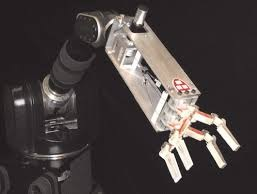
\includegraphics[scale=0.7]{./images/SDMHand}
  \caption{SDM Hand}
  \label{fig:SDMHand}
	\end{figure}
\begin{figure}[h!]
\centering  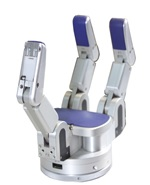
\includegraphics[scale=0.7]{./images/BarrettHand}
  \caption{Barrett Hand}
  \label{fig:BarrettHand}
	\end{figure}
A different approach is to shape the finger surfaces in an anthropomorphic fashion, where the fingertip is round and allows for more flexible manipulation, such as the Robonaut Hand (Fig.\ref{fig:RobonautHand}), and the Shadow Dextrous Hand (Fig.\ref{fig:ShadowDextrousHand}).\\
\begin{figure}[h!]
\centering  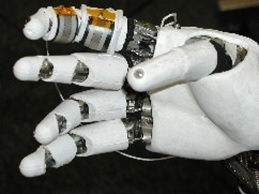
\includegraphics[scale=0.6]{./images/RobonautHand}
  \caption{Robonaut Hand}
  \label{fig:RobonautHand}
	\end{figure}
\begin{figure}[h!]
\centering  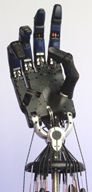
\includegraphics[scale=0.7]{./images/ShadowDextrousHand}
  \caption{Shadow Dextrous Hand}
  \label{fig:ShadowDextrousHand}
	\end{figure}
Finally, some hands have fingers with more generic round surfaces in cylindrical and spherical shapes such as the CyberHand (Fig.\ref{fig:CyberHand}).\\
\begin{figure}[h!]
\centering  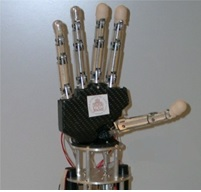
\includegraphics[scale=0.7]{./images/CyberHand}
  \caption{CyberHand}
  \label{fig:CyberHand}
	\end{figure}
Using flat finger pads can often increase the stability of grasps compared to a rounded geometry, but it may also prevent the fingers from being used effectively at a wide range of angles.\\
However, there is little information on how the finger should be shaped in order to facilitate manipulation. There is a lack of studies on what finger surfaces are actually used during manipulation. This is likely due to the difficulty of effectively instrumenting the contact surfaces of the finger pads.\\
%%%%%%%%%%%%%%%%%%%%%%%%%%%%%%%%%%%%%%%%%%%%%%%%%%%%%%%%%%%%%%%%%%%%%%%%%%%%%%%%
\section{\textbf{Traditional and Compliant Joints}}
The number of joints per finger in anthropomorphic robotic hands is extremely important since it provides the hand with conformance to shapes and acts as a contact surface for gripping and support structure for grasps.\\
There are two types of joint designs that have been widely used in robotic hands \cite{siciliano2016springer}. The first type uses standard mechanical components such as hinges, linkages, or gears and belts. Many important features have been achieved in this kind, including high degrees of modularity, built-in actuators, but it involves considerable systems-level complexity and implementation costs.\\
An alternative approach to traditional joints is the compliant joints. These types reduce overall complexity of the robotic hand's mechanisms and hands are able to withstand large impacts without damage. In addition, the advent of new materials and new technologies (e.g. Rapid Prototyping) largely encourages the development of this concept (Fig.\ref{fig:teflon}) (Fig.\ref{fig:springs}) (Fig.\ref{fig:RapidPrototyping}).\\
But it has also some disadvantages. The Range-of-Motion is limited. The Axis Drif; most compliant joints undergo imprecise motion as the center of rotation does not remain fixed with respect to the links it connects. And such joints can suffer Stress Concentration.\\
\begin{figure}[h!]
\centering  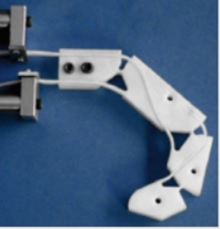
\includegraphics[scale=0.7]{./images/teflon}
  \caption{The finger is obtained in a single teflon piece}
  \label{fig:teflon}
	\end{figure}
\begin{figure}[h!]
\centering  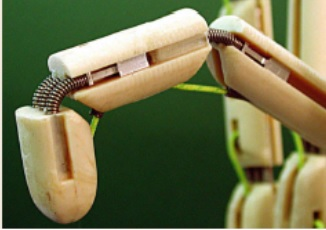
\includegraphics[scale=0.6]{./images/springs}
  \caption{Joint compliance is achieved with metallic springs}
  \label{fig:springs}
	\end{figure}
\begin{figure}[h!]
\centering  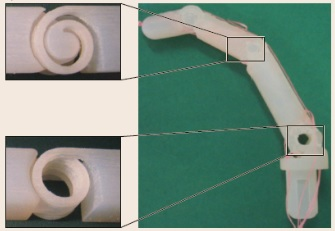
\includegraphics[scale=0.6]{./images/RapidPrototyping}
  \caption{Rapid prototyping allows for different compliant mechanisms as joints}
  \label{fig:RapidPrototyping}
	\end{figure}
%%%%%%%%%%%%%%%%%%%%%%%%%%%%%%%%%%%%%%%%%%%%%%%%%%%%%%%%%%%%%%%%%%%%%%%%%%%%%%%%
\section{\textbf{Built-in Actuation}}
In order to actuate the joints of a robotic finger, two basic approaches for the placement of the actuators are used \cite{belter2013mechanical}:\\
\begin{itemize}
	\item Placing the motors as close as possible to each joint, directly in the fingers and sometimes integrating them within the joint itself (Fig.\ref{fig:VincentFinger}).
	\item Placing the motors into the palm or in the forearm; in this case motion is transmitted to each joint by means of (complex) kinematic chains. (Fig.\ref{fig:MichelangeloDriveMechanism})\\
\begin{figure}[h!]
\centering  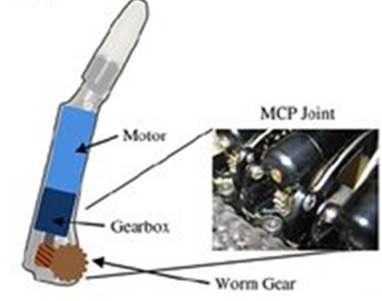
\includegraphics[scale=0.6]{./images/VincentFinger}
  \caption{Vincent finger motor (Vincent Systems) is housed in proximal phalange and rotates worm against fixed worm gear to flex finger.}
  \label{fig:VincentFinger}
	\end{figure}
\begin{figure}[h!]
\centering  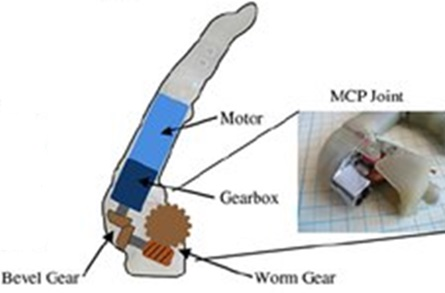
\includegraphics[scale=0.6]{./images/iLimbFinger}
  \caption{iLimb finger (Touch Bionics) is actuated in same manner as Vincent finger but uses set of bevel gears between motor and worm drive. MCP = metacarpal phalange.}
  \label{fig:iLimbFinger}
	\end{figure}	
	\begin{figure}[h!]
\centering  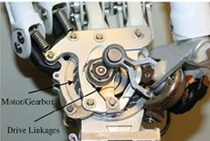
\includegraphics[scale=0.7]{./images/MichelangeloDriveMechanism}
  \caption{Drive mechanism of Michelangelo hand (Otto Bock). Center drive element controls flexion of all four fingers and thumb. Second motor (which actuates against bronze worm gear) independently controls abduction/adduction of thumb.}
  \label{fig:MichelangeloDriveMechanism}
	\end{figure}
\end{itemize}
This built-in actuation simplifies the mechanical configuration of the joint, reducing the transmission chain complexity. It also has the advantage that the motion of the joint is kinematically independent with respect to other joints. However, the motors occupy a large room inside the finger structure, making it harder to host other elements, like sensors or compliant skin layers.\\
%%%%%%%%%%%%%%%%%%%%%%%%%%%%%%%%%%%%%%%%%%%%%%%%%%%%%%%%%%%%%%%%%%%%%%%%%%%%%%%%
\section{\textbf{Transmission}}
Remote actuation is an alternative solution to in-site actuation. In remote actuation, the joint is driven by actuators placed outside the links connected by the joint itself. This kind of systems can be classified according to the type of adopted transmission elements:\\
\begin{itemize}
\item \textbf{Flexible Link Transmission}
	\begin{itemize}
		\item Pulley-routed flexible elements (tendons, chains, belts)
		\item Sheath-routed flexible elements (mainly tendon-like elements)\\
	\end{itemize}
This kind allows the actuators to be located remotely from the joints. Consequently reducing the dimensions and weight of the fingers. But the disadvantage of the flexible cables or flat bend transmission is that they can only be used to pull. In order to achieve the active two-way control a pair is required and this increases the complexity.\\ 
\item \textbf{Rigid Link Transmission}
	\begin{itemize}
		\item Parallel and nonparallel axes gear trains, like bevel gears, worm gears, and so on.\\
	\end{itemize}
\end{itemize}
This kind gives the best stiffness properties to the transmission. Additionally such transmissions require less maintenance than the flexible kind and they allow bidirectional control of the joint. The disadvantage here is that using rigid transmission systems increases the weight, complexity and sometimes dimensions of the hand.\\
Considering the transmission types used in robotic hands developed since 1983 (Fig.\ref{fig:TransmissionsTypes}) we find out that the preferred transmission type is tendons. They allow to simplify the design and to take the actuators off of the hand. However the disadvantage is that they introduce errors. The second most used type is gears, they have more accuracy but also more friction. The direct transmission type is the less used type because of the difficulty in its design.\\
A brief comparison \cite{balasubramanian2014human} based on different parameters, between the main transmission mechanisms that can be employed in artificial hands, is shown in (Fig.\ref{fig:parameters}).\\
\begin{figure}[h!]
\centering  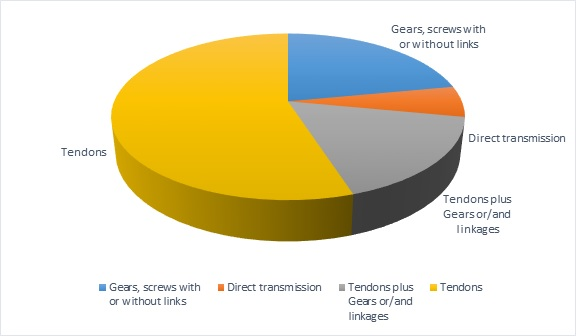
\includegraphics[width=1.0\linewidth]{./images/TransmissionsTypes}
  \caption{Transmissions Types}
  \label{fig:TransmissionsTypes}
	\end{figure}
\begin{figure}[h!]
\centering  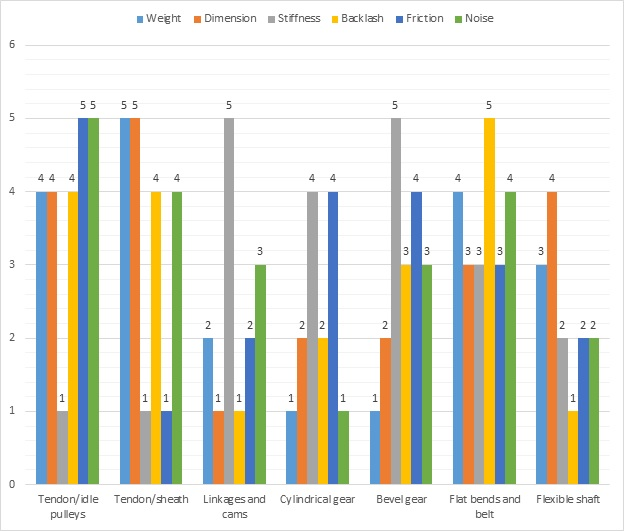
\includegraphics[width=1.0\linewidth]{./images/parameters}
  \caption{Comparison between the main transmission mechanisms}
  \label{fig:parameters}
	\end{figure}
%%%%%%%%%%%%%%%%%%%%%%%%%%%%%%%%%%%%%%%%%%%%%%%%%%%%%%%%%%%%%%%%%%%%%%%%%%%%%%%%
\section{\textbf{Sensors}}
In robotics sensors can be classified in two main categories: Proprioceptive and Exteroceptive sensors.\\
The first type of sensors measures physical information related to the state of the device itself (e.g., position, velocity, and so on), while the second one is devoted to the measurement of data related to the interaction with objects/environment (e.g., applied forces/torques, friction, shape, and so on).\\
Tactile sensing is an essential element of autonomous dexterous robot hand manipulation. It provides information about forces of interaction and surface properties at points of contact between the robot fingers and the objects.\\
In general, the types of information that may be obtained from a tactile sensor are:\\
\begin{itemize}
	\item \textbf{Contact:} This is the most simple information given by the sensor, concerning the presence or absence of a contact.
	\item \textbf{Force:} Each sensing element provides an information related to the amount of locally applied force, which can be used in several manners for successive elaborations.
	\item \textbf{Simple geometrical information}, i. e., position of the contact area, geometrical shape of the contact itself (planar, circular, and so on).
	\item \textbf{Main geometrical features} of the object: By proper elaborations of the data of the taxels, it is possible to deduce the type of object in contact with the sensor, for example a sphere, a cylinder and so on (data relative to the 3-D (three-dimensional) shape).
	\item \textbf{Mechanical properties}, such as friction coefficient, roughness, and so on. Also thermal properties of the object may be measured by a tactile sensor.
	\item \textbf{Slip condition}, i. e., the relative movement between the object and the sensor.
\end{itemize}
As proposed by \cite{yousef2011tactile} the minimum functional requirements for a robotic tactile sensing system mimicking human manipulation is summarized as:\\
		\begin{itemize}
			\item Detect the contact and release of an object.
			\item Detect lift and replacement of an object.
			\item Detect shape and force distribution of a contact region for object recognition.
			\item Detect contact force magnitude and direction for maintaining a stable grasp during manipulation.
			\item Detect both dynamic and static contact forces.
			\item Track variation of contact points during manipulation.
			\item Detect difference between predicted and actual grip forces necessary for manipulation.
			\item Detect force and magnitude of contact forces due to the motion of the hand during manipulation.
			\item Detect tangential forces due to the weight and shape of the object to prevent slip.
			\item Detect tangential forces arising from variations in object parameters (e.g. surface friction, elasticity, etc.) to prevent slip.\\
		\end{itemize}
Most common tactil sensor configurations are:
		\begin{itemize}
			\item Resistive sensors
			\item Piezoelectric sensors
			\item Capacitative sensors
			\item Magnetic transduction sensors
			\item Photoelectric, or optical, tactile sensors\\
		\end{itemize}
Main tactile sensors are presented in the Table \ref{TactilSsensor} \cite{wettels2014multimodal}.\\
\begin{portrait}
\begin{table}[]
\centering
\caption{Summary of tactile sensing technologies}
\label{TactilSsensor}
\begin{tabular}{lll} %{p{1.5cm}p{2cm}p{2cm}}
\hline
\textbf{Transduction Method} & \textbf{Advantages} & \textbf{Disadvantages} \\ \hline
Capacitive & Can be flexible, wide dynamic range, sensitive & Hysteresis, noise, limited resolution \\ \hline
Inductive & High sensitivity, repeatability & Complex construction, electronics in workspace, low spatial resolution \\ \hline
Resistive: deformable contact area & Flexible, thin & Hysteresis \\ \hline
Resistive: conductive fabric & Flexible, robust, simple & Unable to resolve more than one contact point \\ \hline
Resistive: quantum tunneling composite & Sensitive, wide dynamic range & Hysteresis, gas absorption \\ \hline
Resistive: strain gauge & Sensitive, wide dynamic range & Bulky, expensive \\ \hline
Resistive: piezoresistive conductive polymer & Thin, low cost, simple & Hysteresis, stiff \\ \hline
Resistive: piezo-MEMS & Small, multi-element & Large number of wires in workspace \\ \hline
Resistive/Capacitive: liquid channels embedded in elastomer & Small, flexible, multidimensional force sensing capability & Large number of wires in workspace \\ \hline
Polymer-MEMs (multi-modal) & Measures 6-DOF force, heat-flow, temperature, roughness & Large number of wires in workspace, wiring complexity \\ \hline
Piezoelectric & Detects dynamics for slip and texture & Only detects dynamic events, thermal sensitivity \\ \hline
Optical: video processing & Very high resolution, sensitive & Computationally intensive, sensitive to ambient light \\ \hline
Optical: resistive & Flexible, low hysteresis & Complex fabrication \\ \hline
Magneto-elastic & Very sensitive, low hysteresis & Sensitive to external magnetic fields \\ \hline
Magneto-resistive & Robust, sensitive, low hysteresis & Noisy \\ \hline
Ultrasound & Can resolve static and dynamic information & High voltage, complex electronics \\ \hline
\end{tabular}
\end{table}
\end{portrait}
%%%%%%%%%%%%%%%%%%%%%%%%%%%%%%%%%%%%%%%%%%%%%%%%%%%%%%%%%%%%%%%%%%%%%%%%%%%%%%%%
\section{\textbf{Materials and Manufacturing}}
The design and fabrication of a prototype using traditional machinery techniques is a rather long and expensive process, and often the employment of rapid prototyping techniques provides several advantages. One of the main advantages is represented by the chance to develop parts with complex geometry that could not be manufactured using traditional techniques.\\
Won et al. \cite{won2000fabrication} developed a five-finger anthropomorphic hand by using a Selective Laser Sintering technique (SLS) (Fig.\ref{fig:SelectiveLaserSintering}), which allows joints to be manufactured in one-step without requiring assembly. The main drawback of SLS is the lack of mechanical proprieties (such as stiffness and strength), moreover it fails when dimension tolerances are narrowed.\\
\begin{figure}[h!]
\centering  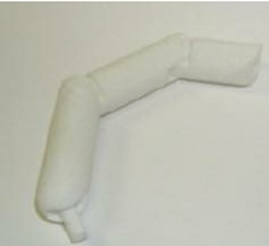
\includegraphics[scale=0.7]{./images/SelectiveLaserSintering}
  \caption{Selective Laser Sintering (SLS)}
  \label{fig:SelectiveLaserSintering}
	\end{figure}
Dalley et al. \cite{dalley2009design} developed a transradial anthropomorphic hand, in which the parts were physically realized in high-strength, nickel-coated thermoplastic using an additive directly incorporated during the manufacturing process (Fig.\ref{fig:NickelCoated}); this method combines the flexibility of the rapid technique with the strength/stiffness of the metallic material. The main drawbacks of this method are the low fatigue resistance, and poor surface finish and geometrical tolerance that often requires re-machining by traditional methods.\\
\begin{figure}[h!]
\centering  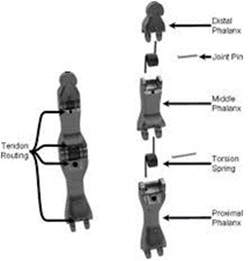
\includegraphics[scale=0.7]{./images/NickelCoated}
  \caption{High-strength, nickel-coated thermoplastic}
  \label{fig:NickelCoated}
	\end{figure}
Dollar and Howe \cite{dollar2010highly} showed how a further integration of sensors, electronics and actuation could be obtained using polymer-based Shape Deposition Manufacturing (SDM) (Fig.\ref{fig:ShapeDepositionManufacturing}). Another advantage of the SDM technique is the possibility of simultaneously creating rigid links and compliant joints of the fingers, providing the hand with passive mechanical compliance useful for grasping in unstructured environments.\\
\begin{figure}[h!]
\centering  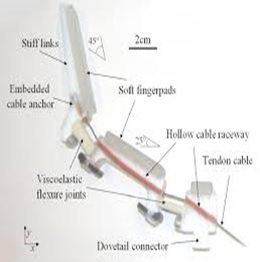
\includegraphics[scale=0.7]{./images/ShapeDepositionManufacturing}
  \caption{Polymer-based Shape Deposition Manufacturing (SDM)}
  \label{fig:ShapeDepositionManufacturing}
	\end{figure}
The use of compliant materials in manufacturing of joints allows a number of components to be avoided (such as pulleys, axis, torsion springs, and so on) and the ability to embed the extension system, disguised as releasing springs, in the structure thus resulting in a reduction in joint size. Examples of artificial hands exploiting compliant joints based on these principles were developed at the University of Bologna, Stanford, Genoa, Scuola Superiore Sant’Anna, and University of Iowa.\\
%%%%%%%%%%%%%%%%%%%%%%%%%%%%%%%%%%%%%%%%%%%%%%%%%%%%%%%%%%%%%%%%%%%%%%%%%%%%%%%%
\section{\textbf{Conclusion and Future Trends}}
In this paper robotic fingers were discussed, their design considerations in choosing the suitable configuration, mechanism and sensors was discussed by considering several projects from past decades to the present. The growing use of the hands in human used environments and the emphasis on sensor development and new materials in the past years, hints that sensors and the use of soft and compliant materials will be the major research approaches in robotic fingers \cite{spiers2018variable}.\\
Another future trend is the development of artificial skins for the fingers with denser spatial resolution and a multitude of sensor modalities, as recent advances in biofabriction techniques could integrate engineered muscle tissues with artificial devices, leading to biohybrid robotics \cite{feinberg2015biological} \cite{morimoto2018biohybrid}.\\
Also as more and more sensors are being employed in smart-phones, which has a big market, will drive down the costs of these sensors and encourage their use in the artificial hand.\\
It is also believed that there is a need for standardization as it is seen of great importance not only for commercial purposes but also for classification of the newly developed devices \cite{ramirez20173}.\\
%%%%%%%%%%%%%%%%%%%%%%%%%%%%%%%%%%%%%%%%%%%%%%%%%%%%%%%%%%%%%%%%%%%%%%%%%%%%%%%%
\begin{landscape}
\begin{table}[]
\centering
\caption{Hand comparison chart from 1979 to 2016.}
\label{hand-comparison}
\begin{tabular}{p{2cm}p{4cm}lp{2cm}p{2cm}lllp{2cm}lll}
\hline
\multicolumn{1}{c}{\textbf{Name}} & \multicolumn{1}{c}{\textbf{Sensors}} & \multicolumn{1}{c}{\textbf{Fingers}} & \multicolumn{1}{c}{\textbf{Transmission}} & \multicolumn{1}{c}{\textbf{Research Institute}} & \multicolumn{1}{c}{\textbf{Year}} & \multicolumn{1}{c}{\textbf{DOF}} & \multicolumn{1}{c}{\textbf{DOA}} & \multicolumn{1}{c}{\textbf{Actuators}} & \multicolumn{1}{c}{\textbf{Weight {[}Kg{]}}} & \multicolumn{1}{c}{\textbf{Load {[}Kg{]}}} & \multicolumn{1}{c}{\textbf{Load {[}N{]}}} \\ \hline
Okada Hand & Potentiometers & 3 & Tendons & & 1979 & 11 & & DC Motors & & & \\ \hline
Stanford/JPL Hand & Tactile Sensors, Tension tendons sensors & 3 & Tendons & Stanford University & 1983 & 9 & 9 & Electrical (DC) & 1.1 &  & 110.8 \\ \hline
Utah/MIT & Hall effect sensors, Tendon tension sensors, tactile distributed sensors & 4 & Tendons & Utah University & 1985 & 16 & 16 & Pneumatic Cylinders & 9 & 9 &  \\ \hline
Belgrade/USC Hand & Potentiometers as positions sensors, Force resistors & 5 &  & Belgrade University & 1988 & 15 & 4 & Electrical Motors &  & 2.26 &  \\ \hline
BarrettHand & Optical Encoders, Tactile sensors & 3 & Tendons, worm gears & Barret Technology Inc. & 1988 & 8 & 4 & Electrical Brushless motors & 1.2 & 6 &  \\ \hline
DLR Hand I & 28 Sensors on each finger, hall sensors, optical position sensor, torque sensor, force sensor, tactile sensors and stereo camera & 4 & Tendons & DLR-German Aerospace Center & 1997 & 16 & 12 & Electrical &  &  &  \\ \hline
Dist Hand & Rotation sensors in each joint & 5 & Tendons & Genova University & 1998 & 16 & 16 & Electrical & 1 &  & 1.96 \\ \hline
Robonaut Hand & 42 sensors plus tactile sensors & 5 & Tendons & NASA Johnson Space Center & 1999 & 19 & 14 & Electrical Brushless Motors &  & 9 &  \\ \hline
Gifu Hand & Magnetic encoder in the motors shaft and tactile distributed sensor & 5 & Gears , Links & Gifu University & 1999 & 20 & 16 & DC Micromotors & 1.4 & 1.83 &  \\ \hline
Robotiq 3 Finger Gripper & current sensor, position sensor, grip sensor & 3 & gears and links & Laval University & 1999 & 10 & 4 & DC Motors & 2.3 & 10 &  \\ \hline
Blackfingers & Position and force sensors directly on the actuator & 5 & Tendons & Politecnico de Milano & 2000 & 22 & 36 & Mckibben Actuators &  &  &  \\ \hline
\begin{tabular}[c]{@{}l@{}}Tuat/Karlsruhe\\   Hand\end{tabular} &  & 5 & Tendons & Tokyo and Karlsruhe Universities & 2000 & 24 & 1 & Electrical & 0.49 &  &  \\ \hline
Ultralight Hand &  & 5 & NONE & Research Center of Karlsruhe & 2000 & 18 & 13 & Flexible Fluidic actuators & 0.2 & 1.22 &  \\ \hline
Variable Force Hand &  & 5 & Tendons & Hokkaido University & 2000 & 10 & 5 &  &  &  &  \\ \hline
DLR Hand II & Torque sensors in each joint & 4 & Tendons & DLR-German Aerospace Center & 2001 & 17 & 13 & Electrical & 2.2 & 3.059 &  \\ \hline
RTR Hand I & Hall effect sensors, strain gages as force sensors & 3 & Screws & Centro INAIL RTR, Scuola Superiore Santa Anna & 2001 & 9 & 3 & DC Micromotors &  &  &  \\ \hline
Dexterous Robot &  & 4 & Tendons & Maryland University & 2001 & 12 &  &  &  &  &  \\ \hline
Shadow EDC Hand & Hall effect sensors, Tactile sensors & 5 & Tendons & Robot Shadow Company Ltd. & 2002 & 23 & 23 & Pneumatic muscles & 4 &  &  \\ \hline
Thinh Hand & Bend Sensors, Camera for visual control of the thumb pronation angle & 4 & Tendons & Florida University & 2002 & 14 & 6 & Electrical &  &  &  \\ \hline


\end{tabular}
\begin{flushright}
\textit{(continued)}
\end{flushright}
\end{table}
\end{landscape}

\begin{landscape}
\begin{table}[]
\begin{flushleft}
{\normalsize Table \ref{hand-comparison} \textit{(Continued)}.}\\
\end{flushleft}
\centering
%\caption{(Continued).}
\label{my-label}
\begin{tabular}{p{2cm}p{4cm}lp{2cm}p{2cm}lllp{2cm}lll}
\hline
\multicolumn{1}{c}{\textbf{Name}} & \multicolumn{1}{c}{\textbf{Sensors}} & \multicolumn{1}{c}{\textbf{Fingers}} & \multicolumn{1}{c}{\textbf{Transmission}} & \multicolumn{1}{c}{\textbf{Research Institute}} & \multicolumn{1}{c}{\textbf{Year}} & \multicolumn{1}{c}{\textbf{DOF}} & \multicolumn{1}{c}{\textbf{DOA}} & \multicolumn{1}{c}{\textbf{Actuators}} & \multicolumn{1}{c}{\textbf{Weight {[}Kg{]}}} & \multicolumn{1}{c}{\textbf{Load {[}Kg{]}}} & \multicolumn{1}{c}{\textbf{Load {[}N{]}}} \\ \hline
High Speed Multifingered Hand & Strain gages, Camera for image processing & 3 & Miniharmonic drive, bevel gears & Tokyo and Hiroshima Universities & 2003 & 10 & 10 & Electrical & 0.8 & 2.85 &  \\ \hline
SMA Hand & Planed to have Position Sensors, Force Sensors and Touch Sensors & 4 & Shape Memory Alloy Wires & State University of New Jersey & 2004 & 14 &  & Electrical & 1.3 & 3.6 &  \\ \hline
ARMAR Hand & Angle sensors, Force Sensors and Pressure Sensors & 5 & Flexible Fluidic Actuators & University of Karlsruhe & 2005 & 8–18 & 8–16 & Micro Gear Pump & 0.49 & 11.21 &  \\ \hline
UB Hand III v1 & Strain=gauge based sensors, position sensors, tendon force sensors & 5 & Elastic Hinges with Tendons & University of Bologna & 2005 & 20 & 16 & DC Brushed Motors &  &  &  \\ \hline
RL1 Hand & Tendon Tension through mathematical approximation & 3 & Tendons & Universidad Carlos III de Madrid & 2006 & 8 & 1 & DC Motors & 0.25 & 2 &  \\ \hline
AAA Hand & External optotrank (Infrared optical device) & 3 & Tendons & Scuola Superiore Santa Anna & 2007 & 10 & 4 & DC Motors & 0.25 & 3.56 &  \\ \hline
FRH-4 Hand & Position Sensors, Tactile Sensors & 5 & Flexible Fluidic Actuators & Research Center Karlsruhe & 2008 & 11 & 12 & Gear Pump & 0.216 & 11.21 &  \\ \hline
IH2 Azzurra & Tendon Force Sensors, 2 Axis fingertip force sensor & 5 & Tendons & Prensilia & 2008 & 11 & 5 & Electric Motors & 0.6 & 10.2 &  \\ \hline
UB Hand III v2 & Optical angular sensors, Optical Tensor Sensors, Strain gauge tension sensors & 5 & Tendons & Bologna University & 2009 & 20 &  & Mckibben Artificial Muscles &  &  &  \\ \hline
TH-3R Hand &  & 5 & Gears, Racks & Tsinghua University & 2009 & 15 & 4 & Motors &  &  &  \\ \hline
Columbia Hand & Position Sensors, Tactile Sensors & 3 & Tendons & Columbia University & 2011 & 9 & 2 & Motors &  &  &  \\ \hline
The Handroid &  & 5 & Tendons & ITK Company & 2011 & 16 & 5 & DC Motors & 0.725 &  &  \\ \hline
KYTECH Hand & Position Sensor & 4 & Gears & Korea Institute of Industrial Technology & 2012 & 16 & 16 & DC Motors & 0.9 & 1.5 &  \\ \hline
The PISA/IIT Soft Hand &  & 5 & Tendons, Rolling cylinders & University of Pisa & 2012 & 18 & 1 & Electric Motor &  &  &  \\ \hline
TDM Hand & No sensors, force approximation using Ozawa and Moriya technique & 3 & Tendons & Ritsumeikan University & 2013 & 12 & 12 & DC Motors &  & 5.1 &  \\ \hline
iHY Robot Hand & Pressure sensors, Optic sensors & 3 & Tendons & Yale and Harvard University & 2014 & 9 & 5 & DC Motors &  & 22 &  \\ \hline
Soft Robotic Hand & Resistive Bend sensors & 3 & Pneumatic tubing & Massachusetts Institute of Technology & 2015 &  &  & Pneumatic piston &  &  &  \\ \hline
HALS &  & 5 & Tendon & Yokohama National U & 2016 & 9 & 5 & DC Motor & 1.2 & 3.059 &  \\ \hline
RBO Hand 2 &  & 5 & Pneuflex & Berlin University of Technology & 2016 & 5 & 7 & Pneumatic & 0.178 & 0.5 &  \\ \hline
UW’s Hand & Joint and Tactile Sensors & 5 & Tendons & University of Washington & 2016 &  & 10 & Servo Motors & 0.942 &  &  \\ \hline
\end{tabular}
\end{table}
\end{landscape}

\listoffigures
\listoftables
\bibliography{./References}
\bibliographystyle{./IEEEtran}
\nocite{*}

%
\end{document}
%
